%%%%%%%%%%%%%%%%%%%%%%%%%%%%%%%%%%%%%%%%%%%%%%%%%%%%%%%%%%%%%%%%%%%%%%%%%%%%%%%%
%                       CHAPTER 4: IMPLEMENTATION DETAILS                      %
%%%%%%%%%%%%%%%%%%%%%%%%%%%%%%%%%%%%%%%%%%%%%%%%%%%%%%%%%%%%%%%%%%%%%%%%%%%%%%%%

\chapter{Implementation Details}\label{section:implementation}

%%%%%%%%%%%%%%%%%%%%%%%%%%%%%%%%%%%%%%%%%%%%%%%%%%%%%%%%%%%%%%%%%%%%%%%%%%%%%%%%
%        SECTION 4.1: BACKEND CORE & ZERO-PLAINTEXT PERSISTENCE                %
%%%%%%%%%%%%%%%%%%%%%%%%%%%%%%%%%%%%%%%%%%%%%%%%%%%%%%%%%%%%%%%%%%%%%%%%%%%%%%%%

\section{Backend Core and Zero-Plaintext Persistence}\label{section:impl-backend}

The backend service runs on Java~21 and Spring Boot~3.3.4. It enforces zero-plaintext storage by ensuring that demographic PII and clinical observations exist exclusively as AES-256-GCM ciphertexts inside PostgreSQL tables, preventing plaintext leakage to database transaction logs, core dumps, or disk swap partitions.

\subsection{Zero-Plaintext JPA Entity Architecture}

In CryptoShred Health, the Java Persistence API (JPA) entities \texttt{Patient} and \texttt{PatientVisit} isolate runtime clinical objects from relational disk tables.

As detailed in Listing~\ref{lst:patient-entity}, all identifiable demographic attributes carry the JPA \texttt{@Transient} annotation. This mapping completely omits fields such as \texttt{firstName}, \texttt{lastName}, \texttt{dateOfBirth}, and \texttt{nhsNumber} from the PostgreSQL DDL schema.

\begin{lstlisting}[language=Java, caption={Zero-plaintext JPA entity implementation in \texttt{Patient.java}.}, label={lst:patient-entity}]
@Entity
@Table(name = "patients", indexes = {
    @Index(name = "idx_patient_blind_nhs", columnList = "blind_index_nhs"),
    @Index(name = "idx_patient_blind_mrn", columnList = "blind_index_mrn"),
    @Index(name = "idx_patient_blind_last_name", columnList = "blind_index_last_name")
})
public class Patient {
    @Id private UUID id;
    @Column(nullable = false, unique = true)
    private String patientId; // Public identifier: PAT-XXXXXXXX

    @Column(columnDefinition = "TEXT") @JsonIgnore
    private String encryptedDataBlob; // Base64 ciphertext package

    @ManyToOne(cascade = CascadeType.ALL)
    @JoinColumn(name = "encryption_key_id") @JsonIgnore
    private EncryptionKey encryptionKey; // Dedicated Vault Transit KEK & wrapped DEK

    // Blind indices for O(1) exact-match database queries
    @Column(name = "blind_index_nhs", length = 64)
    private String blindIndexNhs;

    @Column(nullable = false) private boolean isActive = true;
    @Column(nullable = false) private boolean shredded = false;

    // Transient attributes: decrypted strictly in RAM
    @Transient private String firstName;
    @Transient private String lastName;
    @Transient private String nhsNumber;
    // ... remaining clinical and demographic fields ...
}
\end{lstlisting}

When persisting a patient record, \texttt{PatientService} serializes the in-memory DTO to canonical JSON, passes the byte array to \texttt{EnvelopeEncryptionService}, and stores the resulting Base64 payload in the \texttt{encrypted\_data\_blob} text column. The database schema stores only public UUIDs, encrypted blobs, and blind index hashes.

\subsection{HMAC-SHA256 Blind Indexing Pipeline}

Because relational columns contain zero plaintext, standard SQL queries cannot evaluate search filters on names or national identity numbers. To enable constant-time exact-match lookups without exposing search terms to database administrators, \texttt{CryptoService} implements the deterministic blind indexing pipeline defined in Equation~\ref{eq:blind-index-theory}.

Listing~\ref{lst:blind-index-code} presents the normalization and hashing logic used across all searchable fields:

\begin{lstlisting}[language=Java, caption={Deterministic blind index computation in \texttt{CryptoService.java}.}, label={lst:blind-index-code}]
public String computeBlindIndex(String value, String salt) {
    if (value == null || value.isBlank()) return null;
    byte[] saltBytes = salt.getBytes(StandardCharsets.UTF_8);
    try {
        Mac mac = Mac.getInstance("HmacSHA256");
        mac.init(new SecretKeySpec(saltBytes, "HmacSHA256"));
        byte[] hmac = mac.doFinal(value.trim().toLowerCase().getBytes(StandardCharsets.UTF_8));
        return HexFormat.of().formatHex(hmac);
    } catch (Exception e) {
        throw new IllegalStateException("HMAC-SHA256 blind index computation failed", e);
    } finally {
        Arrays.fill(saltBytes, (byte) 0);
    }
}
\end{lstlisting}

Because demographic inputs (such as fixed-length NHS numbers, MRNs, and bounded surnames) have strictly bounded byte lengths, HMAC-SHA256 digest computation executes in invariant $\mathcal{O}(1)$ time. PostgreSQL maintains standard B-tree indexes over \texttt{blind\_index\_nhs}, \texttt{blind\_index\_mrn}, and \texttt{blind\_index\_last\_name}. When a clinician searches for NHS Number \texttt{485-777-3456}, the backend normalizes the input, evaluates the deterministic HMAC-SHA256 hash in $\mathcal{O}(1)$ time, and dispatches the indexed SQL query shown in Equation~\ref{eq:sql-blind-search}. PostgreSQL executes point lookups via B-tree index scans, resolving record pointers in logarithmic $\mathcal{O}(\log N)$ index traversal time without reading unencrypted demographic data or scanning ciphertext blobs.

\subsection{Scoped Heap Zeroization and Container Memory Pinning}

Garbage-collected runtimes do not guarantee immediate memory wiping when objects leave scope. If raw cryptographic keys remain in JVM heap memory across multiple collection cycles, they are exposed to memory-dump extraction or operating system page swapping.

To eliminate this vulnerability, \texttt{PatientService} enforces scoped byte-array zeroization. All ephemeral Data Encryption Keys and decrypted buffers are manipulated as primitive \texttt{byte[]} buffers inside mandatory \texttt{try-finally} blocks:

\begin{lstlisting}[language=Java, caption={Scoped memory zeroization in \texttt{PatientService.java}.}, label={lst:memory-zeroization}]
byte[] dek = null;
byte[] decryptedBytes = null;
try {
    // 1. Unwrap DEK from Vault Transit KMS
    dek = vaultKmsService.unwrapDek(
            patient.getEncryptionKey().getVaultKeyName(),
            patient.getEncryptionKey().getWrappedDek());

    // 2. Decrypt ciphertext payload with patientId AAD binding
    byte[] aad = patient.getPatientId() != null 
            ? patient.getPatientId().getBytes(StandardCharsets.UTF_8) : null;
    decryptedBytes = envelopeEncryptionService.decrypt(
            patient.getEncryptedDataBlob(),
            patient.getEncryptionKey().getIv(),
            dek,
            aad);

    // ... transient DTO deserialization and processing ...
} catch (Exception e) {
    log.warn("Vault decryption failed for patient {}: key destroyed", patient.getPatientId());
    isShredded = true;
} finally {
    // 3. Scoped zeroization of ephemeral keys and decrypted plaintext in RAM
    if (dek != null) Arrays.fill(dek, (byte) 0);
    if (decryptedBytes != null) Arrays.fill(decryptedBytes, (byte) 0);
}
\end{lstlisting}

Executing \texttt{Arrays.fill(dek, (byte) 0)} and \texttt{Arrays.fill(decryptedBytes, (byte) 0)} immediately overwrites the raw 256-bit symmetric key and decrypted byte arrays with binary zeroes inside the \texttt{finally} block before the method returns. This zeroization of primitive \texttt{byte[]} buffers minimizes the exposure window of raw key material in heap memory. Within managed-runtime engineering constraints, converting decrypted bytes into domain strings (\texttt{new String(decryptedBytes, ...)}) and parsing them via Jackson's \texttt{ObjectMapper} allocates immutable \texttt{String} and DTO objects on the JVM heap. Because Java \texttt{String} instances are immutable and their internal character arrays cannot be wiped without unsafe reflection, these transient domain representations remain governed by standard garbage collection lifecycles until reclaimed and overwritten by HotSpot GC cycles.

The backend is packaged using a multi-stage Docker build: Eclipse Temurin JDK~21 compiles the source code, while the production container executes on a minimal Alpine Linux JRE~21 image run by an unprivileged system user.

Linux kernel memory locking requires an architectural distinction between the KMS engine and Java runtimes. In the HashiCorp Vault container, the \texttt{IPC\_LOCK} capability (\texttt{cap\_add: [IPC\_LOCK]}) is used natively by Vault's Go runtime to execute the POSIX \texttt{mlock()} system call, pinning Vault's in-memory key ring into physical RAM and preventing it from being paged to disk. In the Spring Boot container, however, the HotSpot JVM does not execute \texttt{mlockall()} on heap allocations; granting \texttt{IPC\_LOCK} merely provides the kernel capability without pinning Java heap pages. To eliminate swap leakage for transient JVM objects, swap mitigation is enforced via container host memory management through Docker cgroup memory constraints that disable swap space entirely (\texttt{--memory-swap = --memory} with \texttt{mem\_swappiness = 0}). This ensures that physical host RAM never flushes idle JVM memory pages to unencrypted swap partitions (requirement~SR3).

\subsection{Encrypted Binary File Attachments and Lifecycle Cascading}

Clinical environments routinely generate unstructured binary files, such as diagnostic imaging scans, specialist referral letters, and laboratory discharge summaries in PDF format. Storing these files on conventional filesystem shares risks orphaned data retention and complicates cryptographic erasure. In \textit{CryptoShred Health}, binary files inherit the zero-plaintext database architecture through the \texttt{PatientAttachment} JPA entity and \texttt{AttachmentService}.

Binary files are ingested via multipart HTTP requests (\texttt{POST /api/attachments/visit/\{visitId\}}), requiring \texttt{Role.DOCTOR} or explicit patient ownership authorization. The service unwraps the visit DEK from Vault Transit, encrypts the file byte stream with AES-256-GCM, immediately wipes the in-memory DEK buffer inside a scoped \texttt{finally} block, and persists the resulting Base64 ciphertext alongside non-sensitive metadata (\texttt{fileName}, \texttt{contentType}, \texttt{fileSize}) in the \texttt{PatientAttachment} table. The raw file payload is shielded from accidental JSON serialization via Jackson's \texttt{@JsonIgnore}. When an authorized clinician requests a download (\texttt{GET /api/attachments/\{attachmentId\}/download}), the service unwraps the visit DEK, decrypts the ciphertext in memory, wipes the DEK buffer via \texttt{Arrays.fill(dek, (byte) 0)}, and streams the decrypted binary payload to the HTTP response.

When a clinical encounter or patient profile is crypto-shredded, \texttt{ErasureService} executes a cascading erasure protocol. In PostgreSQL, the service nullifies the attachment ciphertext and IV (\texttt{encrypted\_data\_blob = NULL}, \texttt{iv = NULL}) and marks \texttt{shredded = true}. In cold backup snapshots and WORM archives, the attachment ciphertext remains immutable but becomes mathematically undecryptable ($P \approx 2^{-256}$) because the parent encounter's $\text{KEK}_{\text{visit}}$ is permanently eradicated inside HashiCorp Vault.

\subsection{Policy-Driven Lawful Retention Engine and Distributed Cache Invalidation}

To implement the dynamic retention model (Equations~\ref{eq:active-encounter-set}--\ref{eq:retention-status}), the \texttt{RetentionPolicyService} component tracks hospital-wide statutory retention rules using thread-safe, non-blocking atomic holders. The service encapsulates five concurrent state variables: \texttt{AtomicInteger retentionPeriodYears}, \texttt{AtomicReference<String> regulatoryStandard}, \texttt{AtomicReference<String> description}, \texttt{AtomicReference<LocalDateTime> lastUpdated}, and \texttt{AtomicReference<String> updatedBy}. 

Hospital administrators can adjust statutory retention schedules at runtime via authenticated REST endpoints (\texttt{PUT /api/admin/retention-policy}) without restarting the Spring Boot container. When a new retention duration $Y \in [1, 100]$ is submitted, \texttt{RetentionPolicyService} dynamically derives the applicable regulatory framework:
\begin{itemize}
    \item $Y = 8\text{~years}$: Maps to \texttt{UK\_NHS\_COP\_2021} (NHS Records Management Code of Practice 2021 baseline for general health records).
    \item $Y = 6\text{~years}$: Maps to \texttt{US\_HIPAA\_SEC\_164} (HIPAA Security Rule 45~CFR~\S~164.316(b)(2)(i)).
    \item $Y = 25\text{~years}$: Maps to \texttt{UK\_NHS\_PEDIATRIC\_MATERNITY\_25Y} (NHS pediatric and maternity extended retention rule).
    \item Other values: Assigned to \texttt{CUSTOM\_STATUTORY\_POLICY}.
\end{itemize}

Listing~\ref{lst:retention-service} illustrates the core horizon evaluation and active encounter querying implemented in \texttt{PatientService} and \texttt{PatientVisitRepository}:

\begin{lstlisting}[language=Java, caption={Active encounter querying and rolling retention calculation.}, label={lst:retention-service}]
// 1. Query latest activity strictly over active (non-shredded) visits
@Query("SELECT MAX(v.createdAt) FROM PatientVisit v " +
       "WHERE (v.patient.id = :patientId OR v.patient.patientId = :patientBusinessId) " +
       "AND v.shredded = false")
LocalDateTime findMaxActiveCreatedAtByPatient(@Param("patientId") UUID patientId, @Param("patientBusinessId") String patientBusinessId);

// 2. Evaluate rolling retention boundary
LocalDateTime eligibleDate = latestActivityDate.plusYears(retentionYears);
String retentionStatus = LocalDateTime.now().isAfter(eligibleDate) ? "ELIGIBLE" : "PROTECTED";
\end{lstlisting}

A critical challenge in distributed architectures is preventing stale cache entries from masking updated retention states. When a clinical encounter is cryptographically erased, \texttt{ErasureService} triggers a multi-tier cache invalidation cascade:
\begin{enumerate}
    \item \textbf{Visit Cache Eviction:} The specific encounter is immediately purged from Redis via \texttt{patientVisitCacheService.evict(visitId)}.
    \item \textbf{Patient Demographic Cache Invalidation:} To prevent stale retention statuses from persisting in L2 memory, \texttt{ErasureService} proactively purges the parent patient profile from Redis via \texttt{patientCacheService.evict(patientId)}. Subsequent patient lookups re-query \texttt{findMaxActiveCreatedAtByPatient}, which ignores the newly shredded visit and dynamically recalculates the patient's legal status as \texttt{ELIGIBLE}.
    \item \textbf{Global Policy Mutation Invalidation:} When an administrator reconfigures the retention horizon via \texttt{AdminController}, the service invokes \texttt{patientCacheService.evictAll()}, flushing all \texttt{patient:*} cache keys across the Redis cluster to ensure immediate system-wide compliance consistency.
\end{enumerate}

%%%%%%%%%%%%%%%%%%%%%%%%%%%%%%%%%%%%%%%%%%%%%%%%%%%%%%%%%%%%%%%%%%%%%%%%%%%%%%%%
%        SECTION 4.2: 3-NODE VAULT RAFT KMS & AUTO-FAILOVER                    %
%%%%%%%%%%%%%%%%%%%%%%%%%%%%%%%%%%%%%%%%%%%%%%%%%%%%%%%%%%%%%%%%%%%%%%%%%%%%%%%%

\section{3-Node Vault Raft KMS and Auto-Failover Implementation}\label{section:impl-vault}

Centralized key management is the core operational dependency of the architecture. If the Key Management Service is unavailable, all encrypted clinical records become inaccessible. Conversely, if key destruction is not replicated synchronously across all cluster nodes, a stale replica could decrypt records that were legally erased.

\subsection{Integrated Raft Consensus Storage and Node Bootstrapping}

CryptoShred Health deploys a 3-node HashiCorp Vault cluster running the Raft consensus protocol~\cite{ongaro_raft_2014}. Unlike legacy KMS setups that require external datastores (such as Consul or MySQL), Vault's Integrated Storage engine embeds the Raft consensus state machine directly inside the Vault binary, writing transactions to local append-only Write-Ahead Logs in \texttt{/vault/file}.

Container bootstrapping is orchestrated by an automated startup script (\texttt{vault/entrypoint.sh}). When the cluster boots:
\begin{enumerate}
    \item \textbf{Leader Initialization:} Node~1 checks its initialization status via \texttt{vault status}. If uninitialized, it executes \texttt{vault operator init -key-shares=1 -key-threshold=1 -format=json}, writing the master root token and unseal key to an encrypted runtime volume.
    \item \textbf{Automated Follower Joining:} Nodes~2 and 3 poll Node~1 over the internal Docker network. Once Node~1 is initialized and unsealed, follower nodes join the consensus group via \texttt{vault operator raft join http://vault-1:8200}.
    \item \textbf{Consensus Quorum:} Once the Raft cluster achieves quorum ($N/2 + 1 = 2$ active nodes), the Transit Secrets Engine is mounted at the key path \texttt{transit/}, and the asymmetric proof-signing key is initialized.
\end{enumerate}

\subsection{HAProxy Leader-Routing and Health Monitoring}

While Raft replicates state across all three nodes, cryptographic write operations (such as KEK generation, wrapping, and key destruction) must execute on the active leader node. Standby followers forward write requests across the internal Raft network, introducing unnecessary network hops.

To ensure low-latency routing, an HAProxy reverse proxy acts as the single entry point between Spring Boot and the Vault cluster on port~\texttt{8200}. HAProxy monitors node states using Vault's health API:

\begin{lstlisting}[caption={HAProxy active leader routing configuration (\texttt{vault/haproxy.cfg}).}, label={lst:haproxy-cfg}]
frontend vault_front
    bind *:8200
    default_backend vault_cluster

backend vault_cluster
    mode http
    balance roundrobin
    option httpchk GET /v1/sys/health
    http-check expect status 200
    default-server inter 500ms fall 2 rise 2
    server vault-1 vault-1:8200 check
    server vault-2 vault-2:8200 check
    server vault-3 vault-3:8200 check
\end{lstlisting}

Vault's \texttt{GET /v1/sys/health} endpoint returns HTTP status~\texttt{200} for the active leader, status~\texttt{429} for standby followers, and status~\texttt{503} for sealed nodes. HAProxy evaluates node health every $500\text{~ms}$. If the active leader fails, HAProxy detects the failure within two intervals ($1.0\text{~s}$) and redirects application traffic to the newly elected leader without dropping active clinical transactions.

\subsection{Zero-Plaintext Granular KMS Key Rotation Protocol}

Cryptographic hygiene guidelines (such as NIST SP~800-57~\cite{barker_nist_sp800_57}) mandate periodic key rotation to limit the volume of ciphertext protected under a single key version. Standard re-encryption requires reading ciphertext from storage, decrypting it into memory under the old key, and re-encrypting it under a newly minted key. In an enterprise healthcare deployment, this approach introduces severe CPU bottlenecks, requires extensive database row locks, and exposes bulk clinical plaintext in application heap memory.

\textit{CryptoShred Health} eliminates plaintext exposure by implementing an in-KMS zero-plaintext key rotation protocol orchestrated by \texttt{KeyManagementService} and exposed via \texttt{KeyManagementController} (\texttt{POST /api/keys/rotate}). The controller supports granular rotation across four distinct operational scopes:
\begin{enumerate}
    \item \textbf{Global Scope (\texttt{ALL}):} Iterates through every active encryption key registered in the database, rotating the KEK version and re-wrapping the associated DEK.
    \item \textbf{Patient Scope (\texttt{PATIENT}):} Resolves the patient's demographic master key and all associated clinical visit keys for a specified \texttt{patientId} (\texttt{POST /api/keys/patients/\{patientId\}/rotate}).
    \item \textbf{Visit Scope (\texttt{VISIT}):} Rotates the cryptographic envelope for a single clinical consultation (\texttt{POST /api/keys/visits/\{visitId\}/rotate}).
    \item \textbf{Individual Key Scope (\texttt{KEY}):} Targets a specific key entity by its database primary key (\texttt{keyId}).
\end{enumerate}

Listing~\ref{lst:key-rotation} illustrates the rotation and re-wrapping pipeline implemented in \texttt{KeyManagementService.java}:

\begin{lstlisting}[language=Java, caption={Zero-plaintext DEK re-wrapping in \texttt{KeyManagementService.java}.}, label={lst:key-rotation}]
for (EncryptionKey key : keysToProcess) {
    if (key.isInvalidated()) continue; // Preserve shredded tombstones

    // 1. Advance KEK version inside Vault Transit
    vaultKmsService.rotateKey(key.getVaultKeyName());

    // 2. Re-wrap DEK under new KEK version inside KMS memory (zero plaintext exposure)
    String newWrappedDek = vaultKmsService.rewrapDek(
            key.getVaultKeyName(), key.getWrappedDek());

    // 3. Update persistent key entity metadata
    key.setKeyVersion(key.getKeyVersion() + 1);
    key.setWrappedDek(newWrappedDek);
    key.setRotatedAt(LocalDateTime.now());
    encryptionKeyRepository.save(key);
}
\end{lstlisting}

During re-wrapping, HashiCorp Vault's Transit engine decrypts the DEK under KEK version $v$ and immediately re-encrypts it under version $v+1$ entirely within KMS memory. The plaintext DEK never crosses the network or enters the Spring Boot heap. Keys flagged as shredded (\texttt{invalidated = true}) are automatically skipped with status \texttt{SKIPPED\_INVALIDATED}, ensuring that cryptographic tombstones cannot be re-encrypted or restored to an active state. Advancing the KEK version alone does not prevent older key versions from decrypting legacy ciphertexts; to enforce cryptographic hygiene, \texttt{KeyManagementService} propagates an updated \texttt{min\_decryption\_version} configuration parameter to Vault Transit (\texttt{POST /v1/transit/keys/\{name\}/config}), setting it to the newly minted version $v+1$. This permanently disables decryption under superseded KEK versions directly at the KMS barrier, rendering compromised historical key backups useless. High-level key metrics (total keys, active keys, and shredded tombstones) are monitored via \texttt{GET /api/keys/summary}.

%%%%%%%%%%%%%%%%%%%%%%%%%%%%%%%%%%%%%%%%%%%%%%%%%%%%%%%%%%%%%%%%%%%%%%%%%%%%%%%%
%     SECTION 4.3: POST-QUANTUM HYBRID SIGNING & MERKLE RECONCILER             %
%%%%%%%%%%%%%%%%%%%%%%%%%%%%%%%%%%%%%%%%%%%%%%%%%%%%%%%%%%%%%%%%%%%%%%%%%%%%%%%%

\section{Post-Quantum Hybrid Signing and Merkle Tombstone Reconciler}\label{section:impl-signing}

Verifiable deletion requires undeniable proof that a cryptographic key was permanently destroyed. Because deletion proofs must remain legally defensible over multi-decade retention windows, digital signatures must withstand both classical cryptanalysis and future quantum attacks.

\subsection{Hybrid Classical and Lattice-Based Signing Architecture}

CryptoShred Health implements the dual-signing framework defined in Equation~\ref{eq:hybrid-signature}, combining classical RSA-2048 with the post-quantum Module-Lattice Digital Signature Algorithm (ML-DSA-65)~\cite{nist_fips_204}. The signing subsystem is implemented in \texttt{ProofSigningService.java} using the BouncyCastle Post-Quantum Cryptography provider (\texttt{BCPQC}):

\begin{lstlisting}[language=Java, caption={Post-quantum ML-DSA-65 signature generation in \texttt{ProofSigningService.java}.}, label={lst:pqc-signing}]
public String signPqc(String data) {
    if (pqcKeyPair == null) {
        throw new IllegalStateException("ProofSigningService PQC keypair is not initialized");
    }
    try {
        Signature pqcSig = Signature.getInstance("Dilithium3", "BCPQC");
        pqcSig.initSign(pqcKeyPair.getPrivate());
        pqcSig.update(data.getBytes(StandardCharsets.UTF_8));
        byte[] signatureBytes = pqcSig.sign();
        return Base64.getEncoder().encodeToString(signatureBytes);
    } catch (Exception e) {
        log.error("Failed to generate PQC ML-DSA-65 signature: {}", e.getMessage(), e);
        throw new RuntimeException("Error signing proof artifact with PQC ML-DSA-65", e);
    }
}
\end{lstlisting}

HashiCorp Vault Transit generates the classical signature directly within the isolated KMS using standard 2048-bit RSA (\texttt{SHA256withRSA}). The private RSA key never leaves the KMS boundary. In parallel, the Spring Boot backend generates a 3{,}309-byte post-quantum digital signature over the canonical delimited string representation ($m_{\text{canonical}}$, Equation~\ref{eq:canonical-payload}) of the deletion certificate. Specifically, the prototype implements CRYSTALS-Dilithium3 (standardized by NIST in FIPS~204 as ML-DSA-65) via the BouncyCastle Post-Quantum Cryptography provider (\texttt{BCPQC}) using the algorithm identifier \texttt{"Dilithium3"}.

\subsection{4-Tier Verification Pipeline}

When an auditor or patient submits a deletion certificate for validation, \texttt{ProofVerificationService} executes an exhaustive 4-tier verification protocol:
\begin{enumerate}
    \item \textbf{Tier 1 (Payload Integrity):} The service verifies the SHA-256 integrity digest committing the entity identifier, timestamp, and legal context into leaf hash $H_{\text{leaf}}$, verifying exact byte conformity with canonical payload $m_{\text{canonical}}$ (Equation~\ref{eq:canonical-payload}).
    \item \textbf{Tier 2 (Classical RSA Validation):} The RSA signature is verified against the public key exported by Vault Transit (\texttt{transit/keys/proof-signing-key}).
    \item \textbf{Tier 3 (Post-Quantum ML-DSA Validation):} The ML-DSA-65 signature is verified using BouncyCastle's lattice-vector verification algorithms, ensuring mathematical validity against quantum adversaries.
    \item \textbf{Tier 4 (Directional Binary Merkle Tree Path Reconstruction):} The verification engine traverses the inclusion path stored in the certificate, applying the directional sorted-pair rules defined in Equation~\ref{eq:merkle-directional-calc}.
\end{enumerate}

\begin{figure}[H]
    \centering
    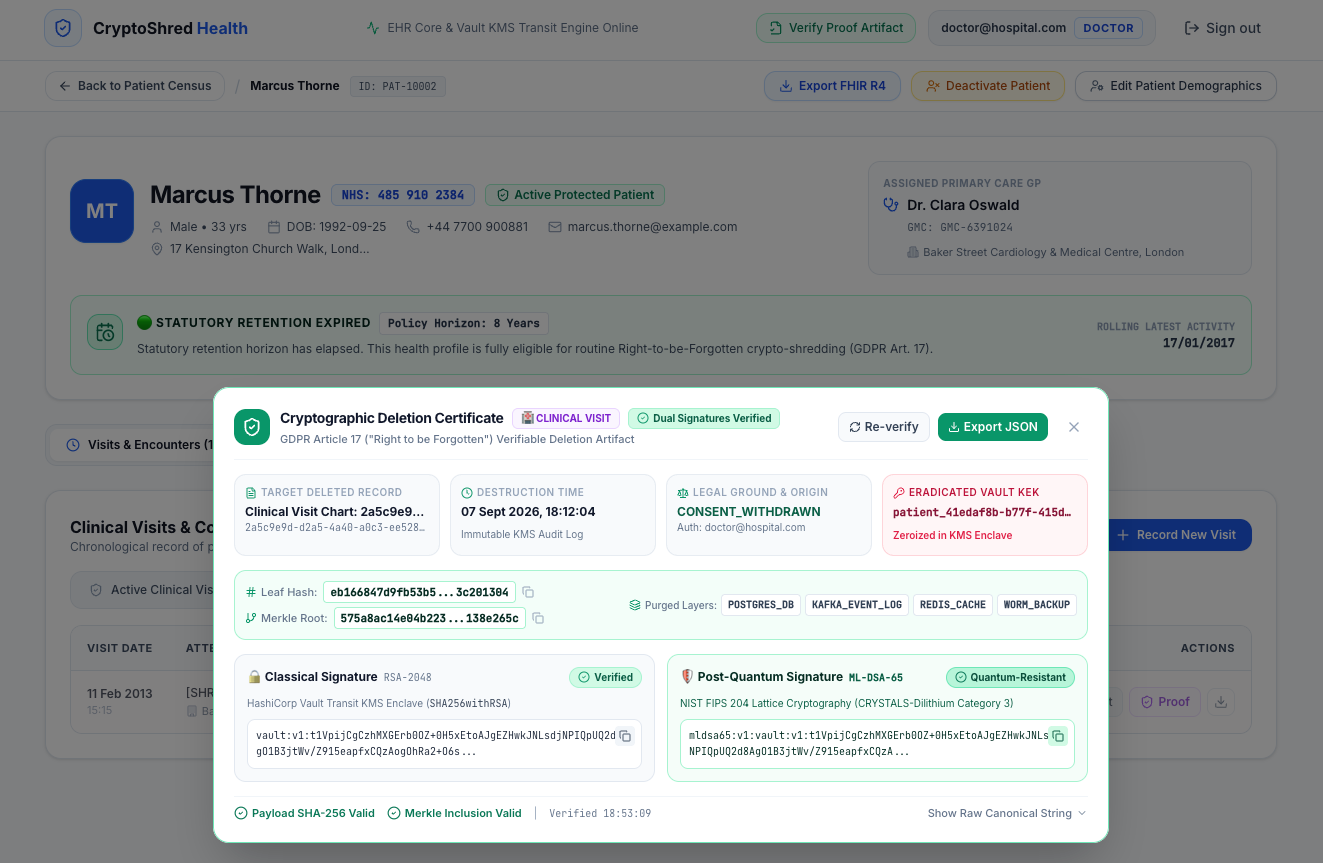
\includegraphics[width=0.95\textwidth]{images/ui_merkle_verifier.png}
    \caption{Interactive cryptographic deletion certificate and Binary Merkle Tree inclusion proof verification interface, displaying the 4-tier validation pipeline and post-quantum ML-DSA-65 digital signature verification.}
    \label{fig:ui-merkle-verifier}
\end{figure}

If the reconstructed hash matches the public Merkle root stored in the database header, the deletion is cryptographically proven to be part of the tamper-evident history.

\subsection{Zero-Trust Offline Public Key Verification}

In regulatory compliance audits, relying on the inspected entity's live backend to verify deletion certificates introduces trust dependencies. An adversary could compromise the application server to spoof verification responses. To ensure zero-trust, air-gapped verifiability, \texttt{ErasureController} exposes the public endpoint \texttt{GET /api/erasure/public-key}.

This endpoint invokes \texttt{ProofSigningService.getPublicKeyPem()} to export the platform's 2048-bit RSA public key formatted as a standard PEM block. Vault Transit generates standard 2048-bit RSA signatures using \texttt{SHA256withRSA}. External Data Protection Officers (DPOs), patient representatives, and legal auditors can download this public key once, disconnect from the network, and verify the classical signature $\sigma_{\text{RSA}}$ on certificate $\mathcal{C}_{\text{erasure}}$ (Equation~\ref{eq:certificate-structure}) using standard OpenSSL tools:
\begin{lstlisting}[language=bash]
openssl dgst -sha256 -verify public-key.pem -signature cert.sig cert_payload.json
\end{lstlisting}
Because the public key is mathematically bound to Vault Transit's internal private key, external parties can establish the authenticity of the deletion receipt and recalculate the Merkle root without accessing or trusting internal hospital microservices.

\subsection{Merkle Tombstone Reconciliation Engine}

To prevent keys from being resurrected after restoring older backup snapshots (Section~\ref{section:kms-ha-tombstone}), \texttt{MerkleTombstoneReconciliationService} runs an automated audit whenever the application starts up. To guarantee resilience against pre-shred ($T_0 < T_1$) database restorations, the service harvests tombstones from two independent locations: relational entity records (\texttt{findByShreddedTrue()}) and external immutable WORM deletion receipts (\texttt{backups/deletion-receipt\_*.json}) read via directory streams (\texttt{Files.newDirectoryStream}). The service gathers all destroyed key identifiers into an aggregated tombstone set $\mathcal{K}_{\text{tombstones}}$ and compares them against Vault's active keys.

Algorithm~\ref{alg:tombstone-reconciler} outlines this reconciliation procedure, which executes during application startup on \texttt{ApplicationReadyEvent} before processing incoming user traffic:

\begin{algorithm}[H]
\caption{Merkle Tombstone Reconciliation and Key Purge}\label{alg:tombstone-reconciler}
\begin{algorithmic}[1]
\Require Active Vault keys $\mathcal{K}_{\text{vault}}$, Database records $\mathcal{D}$, WORM receipt ledger $\mathcal{W}$
\Ensure Detects and purges resurrected encryption keys
\State $\mathcal{K}_{\text{db}} \gets \left\{ \text{KeyOf}(r) \mid r \in \mathcal{D} \land \text{IsShredded}(r) \right\}$ \Comment{Harvest from database}
\State $\mathcal{K}_{\text{worm}} \gets \left\{ \text{KeyOf}(w) \mid w \in \mathcal{W} \right\}$ \Comment{Harvest from WORM receipts}
\State $\mathcal{K}_{\text{tombstones}} \gets \mathcal{K}_{\text{db}} \cup \mathcal{K}_{\text{worm}}$ \Comment{Aggregate immutable tombstones}
\State $\mathcal{K}_{\text{resurrected}} \gets \mathcal{K}_{\text{vault}} \cap \mathcal{K}_{\text{tombstones}}$ \Comment{Identify restored keys}
\ForAll{$k \in \mathcal{K}_{\text{resurrected}}$}
    \State $\text{DestroyVaultKey}(k)$ \Comment{Permanently delete key in Vault Transit}
\EndFor
\State \textbf{return} $|\mathcal{K}_{\text{resurrected}}|$ \Comment{Number of purged keys}
\end{algorithmic}
\end{algorithm}

By running this reconciliation audit on startup before processing user traffic, CryptoShred Health guarantees that restoring an older backup snapshot cannot resurrect previously destroyed encryption keys.

%%%%%%%%%%%%%%%%%%%%%%%%%%%%%%%%%%%%%%%%%%%%%%%%%%%%%%%%%%%%%%%%%%%%%%%%%%%%%%%%
%   SECTION 4.4: IMMUTABLE STREAMING, REDIS CACHE & DISASTER RECOVERY          %
%%%%%%%%%%%%%%%%%%%%%%%%%%%%%%%%%%%%%%%%%%%%%%%%%%%%%%%%%%%%%%%%%%%%%%%%%%%%%%%%

\section{Immutable Streaming, Redis L2 Cache, and Coordinated Disaster Recovery}\label{section:impl-streaming}

Clinical architectures require real-time event distribution across microservices without violating GDPR deletion requirements on distributed event brokers.

\subsection{Kafka KRaft Event Log Streaming and Fail-Safe Consumption}

CryptoShred Health uses Apache Kafka~3.7 running in KRaft mode. All patient lifecycle actions are published to the \texttt{patient-record-events} topic, configured with an immutable one-year retention window ($31,536,000,000\text{~ms}$).

To process high-throughput event streams without race conditions, Kafka splits its audit topic into $N_{\text{partitions}}$ parallel queues (partitions). The backend uses the patient's unique UUID as the message routing key:
\begin{equation}
    \text{Partition}(E) = \text{Hash}(\text{patientId}) \pmod{N_{\text{partitions}}}
    \label{eq:kafka-partition-impl}
\end{equation}
In Equation~\ref{eq:kafka-partition-impl}, taking the hash modulo the number of partitions $N_{\text{partitions}}$ calculates a consistent partition index ($0$ to $N-1$). This mathematical routing guarantees that while different patients are processed in parallel across separate queues, all events for a given patient (from registration to eventual cryptographic shredding) land on the exact same queue in strict chronological sequence.

The system streams nine distinct lifecycle events across three operational boundaries:
\begin{enumerate}
    \item \textbf{Patient Demographic Events:} \texttt{PATIENT\_CREATED} (initial registration), \texttt{PATIENT\_UPDATED} (demographic revisions), \texttt{PATIENT\_DEACTIVATED} (administrative discharge), and \texttt{PATIENT\_ACTIVATED} (chart restoration).
    \item \textbf{Patient Cryptographic Key Operations:} \texttt{PATIENT\_KEY\_ROTATED} (zero-plaintext KEK re-wrapping) and \texttt{PATIENT\_SHREDDED} (irreversible master key destruction under GDPR Article~17).
    \item \textbf{Clinical Encounter Events:} \texttt{VISIT\_CREATED} (consultation intake), \texttt{VISIT\_UPDATED} (vitals/notes amendments), and \texttt{VISIT\_SHREDDED} (granular encounter erasure).
\end{enumerate}

When downstream analytics services consume historical events from Kafka, reading an event from a shredded patient causes Vault Transit decryption to fail because the underlying KEK has been destroyed. \texttt{EventLogConsumer} implements a fail-safe error recovery pattern: when a cryptographic decryption failure is caught during message processing, the consumer logs the expected post-shred condition and handles undecryptable records cleanly rather than crashing or stalling the consumer group.

\subsection{Redis L2 Cache with Shredded-Entity Bypass Filter}

To minimize latency on high-frequency demographic queries, \texttt{PatientCacheService} integrates a Redis~7 caching layer with a default Time-To-Live (TTL) of 15~minutes ($900\text{~s}$).

Standard caching architectures can leak shredded data if records remain cached in Redis after KEK destruction in Vault. CryptoShred Health enforces a two-tier cache invalidation safeguard:
\begin{enumerate}
    \item \textbf{Proactive Cache Invalidation:} During cryptographic erasure, \texttt{ErasureService} explicitly deletes the patient's cache key (\texttt{patient:\{id\}}) from Redis before committing the database transaction.
    \item \textbf{Check-First Shredded Bypass Filter:} When resolving read queries, the backend first checks the database \texttt{shredded} flag. If \texttt{shredded == true}, the application bypasses the Redis cache entirely and immediately returns the redacted response. This ensures that even if an orphaned cache entry persists, no unauthorized client can retrieve it.
\end{enumerate}

\subsection{Atomic Coordinated Backup Engine}

Disaster recovery in an envelope-encrypted architecture requires synchronizing three independent persistence layers: relational database tables, KMS key states, and immutable Write-Once-Read-Many (WORM) audit exports.

To prevent disaster recovery desynchronization, \texttt{BackupManagementService} creates synchronized backup bundles through automated nightly schedules (at 02:00~UTC) and on-demand admin endpoints (\texttt{POST /api/admin/backups/bundle}). 

Because restoring encrypted database records without their exact matching KMS keys leaves data permanently locked, the engine packages both datastores together into a single timestamped archive (\texttt{bundle\_YYYY-MM-DD\_HH-mm-ss/}) containing four synchronized components:
\begin{enumerate}
    \item \textbf{PostgreSQL Database Dump:} A consistent SQL backup of all encrypted tables, entity schemas, and blind indexes generated via \texttt{pg\_dump}.
    \item \textbf{Vault Raft KMS Snapshot:} A point-in-time binary snapshot of the 3-node HashiCorp Vault key cluster generated via the Vault operational API (\texttt{vault operator raft snapshot save}).
    \item \textbf{Immutable WORM Archive:} A JSON export of all clinical encounter records and cryptographic Merkle deletion receipts.
    \item \textbf{Cryptographic Manifest (\texttt{bundle\_manifest.json}):} A master ledger containing SHA-256 integrity hashes for all files in the bundle, dual-signed with both Vault RSA-2048 and post-quantum ML-DSA-65 signatures to guarantee the backup cannot be tampered with.
\end{enumerate}

Restoration is executed via \texttt{scripts/restore-bundle.sh}, which verifies all SHA-256 checksums in the manifest before restoring the database schema, applying the Raft snapshot, and triggering the Merkle Tombstone Reconciler.

\subsection{Auditor WORM Snapshot Verification and Zero-Purge Receipts}

Under GDPR Article~17, hospital compliance officers must verify that cold, immutable backups comply with erasure mandates even when physical Write-Once-Read-Many (WORM) storage prevents file modification or deletion. To prove that historical snapshots contain zero decryptable records, the platform introduces the auditor verification API via \texttt{WormBackupController} and \texttt{WormBackupExporterService}.

The controller provides an audit-grade interface restricted to users with \texttt{Role.AUDITOR} or \texttt{Role.DOCTOR}:
\begin{itemize}
    \item \textbf{Snapshot Export (\texttt{POST /api/backups/export}):} Captures an immediate point-in-time WORM snapshot of all patient encounters, serializing encrypted blobs and wrapped DEKs into an immutable JSON ledger.
    \item \textbf{Snapshot Inspection (\texttt{GET /api/backups/snapshots}):} Lists exported WORM archive files, providing file paths, record counts, and generation timestamps. Detailed snapshot payloads are retrieved via \texttt{GET /api/backups/snapshots/\{fileName\}}.
    \item \textbf{Post-Shred Verification (\texttt{POST /api/backups/verify-shred}):} Validates that a crypto-shredded encounter stored on immutable WORM media cannot be decrypted.
\end{itemize}

When an auditor triggers shred verification for an encounter ID within a target snapshot file, \texttt{WormBackupExporterService} locates the entry, extracts the stored \texttt{vaultKeyName} and \texttt{wrappedDek}, and attempts to unwrap the DEK via \texttt{vaultKmsService.unwrapDek()}. Because the underlying KEK was destroyed in Vault Transit during crypto-shredding, the KMS call throws an exception. The service catches the failure and returns an audit confirmation with status token \texttt{[ZERO\_PURGE\_SUCCESS]}, verifying that the Vault KEK is destroyed and ciphertext on immutable WORM media remains mathematically undecryptable.

If key unwrapping unexpectedly succeeds, the endpoint returns a high-priority warning (\texttt{[WARNING\_DECRYPTION\_SUCCEEDED]}), immediately flagging the anomaly to compliance staff. Upon every cryptographic erasure event, the service writes a standalone WORM deletion receipt (\texttt{deletion-receipt\_*.json}) sealed with POSIX read-only file permissions (\texttt{file.setReadOnly()}) and an embedded SHA-256 fingerprint, guaranteeing an immutable physical audit trail.

%%%%%%%%%%%%%%%%%%%%%%%%%%%%%%%%%%%%%%%%%%%%%%%%%%%%%%%%%%%%%%%%%%%%%%%%%%%%%%%%
%   SECTION 4.5: HEALTHCARE INTEROPERABILITY & OBSERVABILITY                   %
%%%%%%%%%%%%%%%%%%%%%%%%%%%%%%%%%%%%%%%%%%%%%%%%%%%%%%%%%%%%%%%%%%%%%%%%%%%%%%%%

\section{Healthcare Interoperability, Clinical Frontend, and Observability}\label{section:impl-frontend}

Clinical adoption requires strict adherence to healthcare data standards, responsive user interfaces for medical practitioners, and continuous operational observability.

\subsection{HL7 FHIR R4 Bundle Exporter and UK Core Profiles}

To enable interoperability with external hospital systems and national registries, \texttt{FhirController.java} and \texttt{FhirExportService} export patient health records into standard Fast Healthcare Interoperability Resources (HL7 FHIR Release~4) Collection Bundles~\cite{hl7_fhir_r4}.

The exporter maps internal relational models into a suite of official UK Core FHIR profiles:
\begin{itemize}
    \item \textbf{\texttt{UKCore-Patient}:} Formats demographic identifiers, official 10-digit NHS Numbers (\texttt{https://fhir.nhs.uk/Id/nhs-number}), internal Medical Record Numbers (MRN), contact telecom channels, residential addresses, and references to assigned General Practitioners.
    \item \textbf{\texttt{UKCore-Practitioner}:} Represents registered General Practitioners (GPs), encoding General Medical Council (GMC) reference numbers (\texttt{https://fhir.hl7.org.uk/Id/gmc-number}), professional names, and practice telecom details.
    \item \textbf{\texttt{UKCore-Encounter}:} Encapsulates clinical consultations, setting classification to ambulatory (\texttt{AMB}), and recording start timestamps, attending physicians, and chief complaints.
    \item \textbf{\texttt{UKCore-Condition}:} Represents clinical diagnoses and chronic conditions, linking them to encounters and patients. Active records carry \texttt{clinicalStatus = active}; upon cryptographic erasure, the status switches to \texttt{inactive}, and assessment notes are redacted to \texttt{[SHREDDED]}.
    \item \textbf{\texttt{UKCore-Observation}:} Standardizes diagnostic vitals and biometric panels using universal Logical Observation Identifiers Names and Codes (LOINC) and Unified Code for Units of Measure (UCUM).
    \item \textbf{\texttt{UKCore-AllergyIntolerance}:} Documents drug and substance allergies with verification status \texttt{confirmed} and active clinical states.
    \item \textbf{\texttt{UKCore-MedicationStatement}:} Records active clinical prescriptions, dosages, and therapeutic regimens.
    \item \textbf{\texttt{UKCore-DocumentReference}:} Encapsulates clinical attachments (PDFs and diagnostic imaging), recording MIME types, file sizes, creation timestamps, and redaction flags.
\end{itemize}

When exporting records for a crypto-shredded patient, the service strips all PII fields and injects a standard FHIR security tag (\texttt{code: "REDACTED"}, \texttt{system: "http://terminology.hl7.org/CodeSystem/v3-ObservationValue"}, \texttt{display: "Crypto-Shredded under GDPR Art. 17"}). Using the standard \texttt{REDACTED} vocabulary token guarantees strict schema validation across HL7 FHIR R4 validator suites, while preserving human-readable legal semantics for medical compliance auditors.

\subsection{React 19 Clinical Dashboard and Containerized Nginx Delivery}

The frontend is built with React~19, TypeScript, and Tailwind~CSS, bundled via Vite. In production, the client application is packaged using a multi-stage Docker build: a Node~20 builder compiles the TypeScript source into minified static assets, which are transferred to a minimal Nginx~1.27 Alpine web server image.

The Nginx container serves a dual purpose:
\begin{enumerate}
    \item \textbf{Frontend Delivery and Path Routing:} Nginx delivers static React application assets and rewrites deep client routes back to \texttt{index.html}, ensuring client-side React Router navigation resolves consistently without page refresh faults.
    \item \textbf{Internal API Reverse Proxying:} Nginx proxies incoming \texttt{/api/} HTTP requests directly to the internal Spring Boot backend (\texttt{http://backend:8080/api/}) across the isolated Docker bridge network (\texttt{cryptoshred-net}), terminating external traffic while eliminating Cross-Origin Resource Sharing (CORS) overhead in production.
\end{enumerate}

The Primary Care Patient Census dashboard (\texttt{PatientCensusTable.tsx}) organizes patient management into four dedicated views:
\begin{enumerate}
    \item \textbf{Active Patients:} Displays patients with active Vault KMS keys and valid clinical charts.
    \item \textbf{Inactive Patients:} Displays discharged or transferred patients whose records remain encrypted but inactive.
    \item \textbf{Crypto-Shredded Patients:} Displays patients whose KEKs have been destroyed under GDPR Article~17, providing direct access to verifiable deletion certificates.
    \item \textbf{All Patients:} Full clinical registry across all patient states for administrative oversight.
\end{enumerate}

\begin{figure}[H]
    \centering
    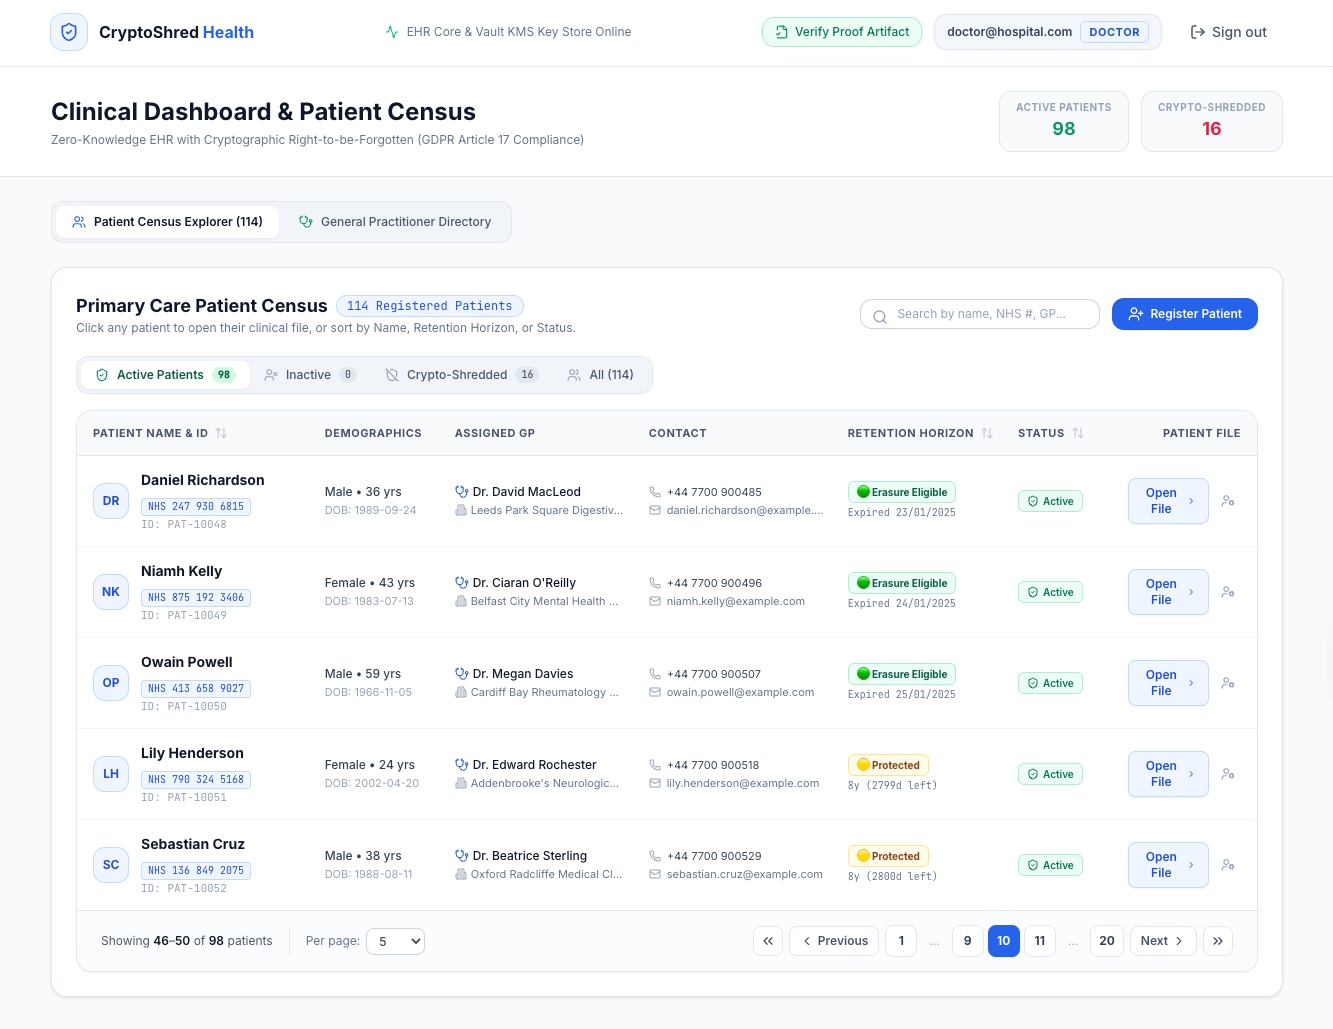
\includegraphics[width=0.95\textwidth]{images/ui_patient_census.png}
    \caption{Primary Care Patient Census dashboard with 5-record pagination view, displaying NHS numbers retrieved using blind indexes, Medical Record Numbers, assigned General Practitioners, and retention status badges.}
    \label{fig:ui-patient-census}
\end{figure}

Role-Based Access Control (RBAC) is enforced through React context providers (\texttt{AuthContext.tsx}). Administrative users can provision medical staff and manage KMS key rotation, doctors can register patients and record clinical visits, while auditors have read-only access restricted to deletion certificates and Merkle proof verification modals.

\begin{figure}[H]
    \centering
    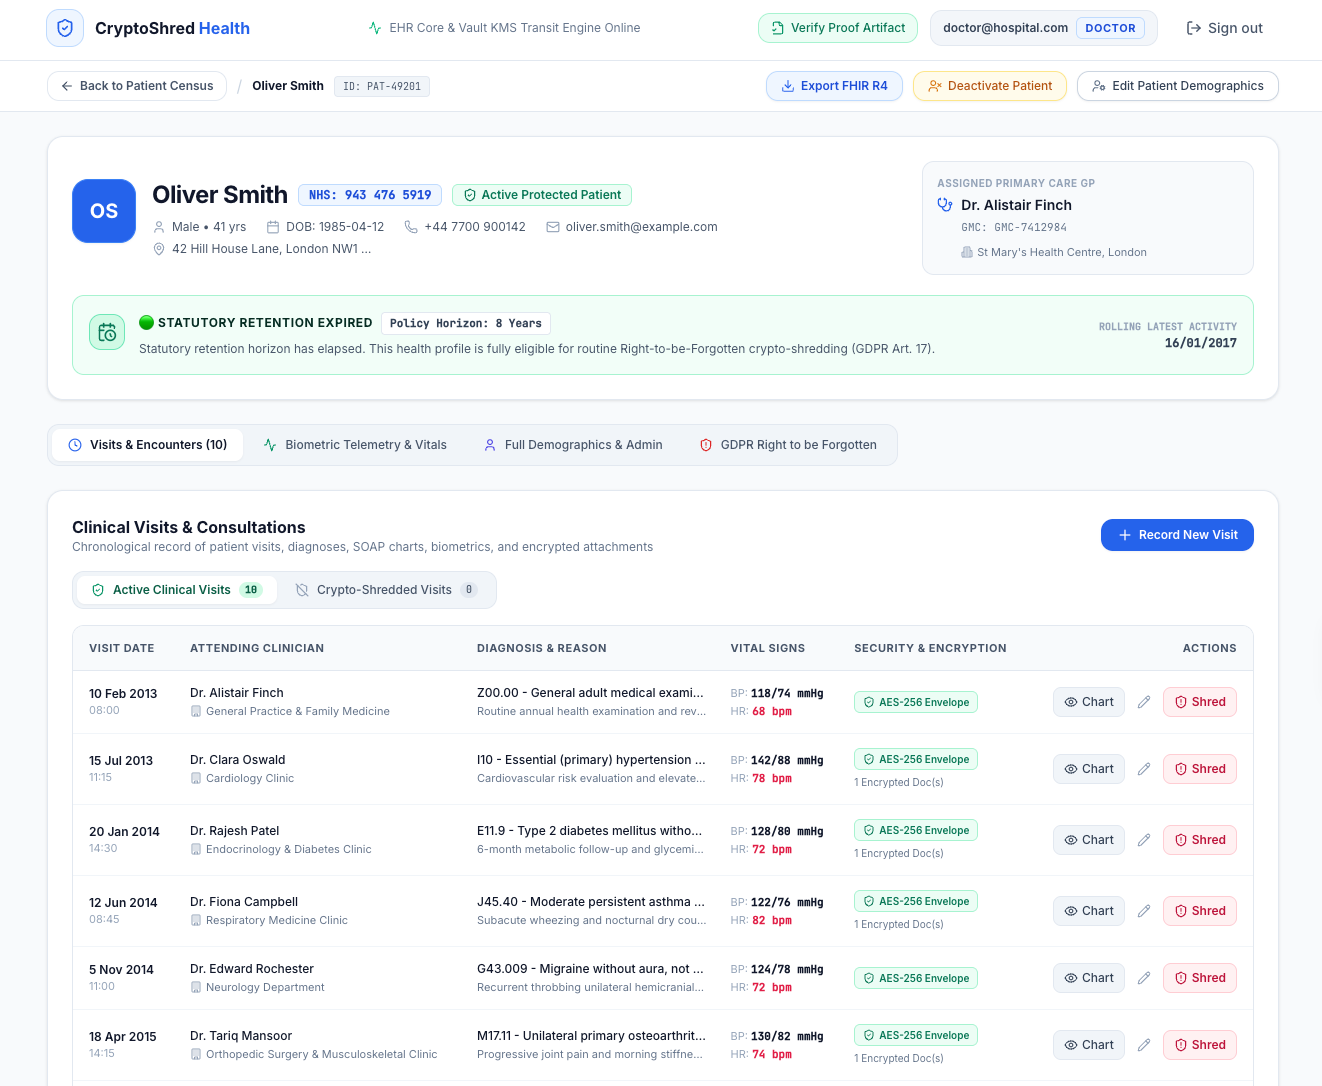
\includegraphics[width=0.95\textwidth]{images/ui_patient_chart.png}
    \caption{Patient clinical chart and consultation view, illustrating master demographic isolation, chronological encounter records, encrypted binary PDF attachments, and the GDPR Article~17 crypto-shredding action interface.}
    \label{fig:ui-patient-chart}
\end{figure}

\subsection{Modular Container Orchestration and Security Network Boundaries}

To isolate infrastructure tiers while supporting flexible evaluation environments, the platform orchestrates containerized services through structured operational profiles:
\begin{enumerate}
    \item \textbf{Core Persistence and KMS Tier (\texttt{default}):} Orchestrates the PostgreSQL~15 database, the 3-node HashiCorp Vault Raft cluster fronted by HAProxy, Apache Kafka~3.7 in KRaft consensus mode, and Redis~7. In production configurations, all datastores bind strictly to private container interfaces on the internal bridge network (\texttt{cryptoshred-net}) with zero public host port exposure (while development Compose manifests expose debug ports for developer tooling).
    \item \textbf{Application and Ingress Tier (\texttt{app}):} Executes the Spring Boot Java~21 application and the Nginx web container, communicating with persistence and KMS engines exclusively over authenticated internal container networks.
    \item \textbf{Observability Tier (\texttt{monitoring}):} Provisions Prometheus and Grafana instances alongside specialized metrics exporters to collect continuous runtime telemetry without interfering with clinical transactions.
\end{enumerate}
This network segmentation enforces the principle of least privilege at the transport layer: external traffic can reach only the Nginx edge gateway, while backend databases, cache instances, and Vault cluster nodes remain isolated from direct host routing.

\subsection{Custom Prometheus Metrics Hierarchy and Observability Architecture}

Operational monitoring is orchestrated using Prometheus and Grafana. While standard Spring Boot Actuator endpoints provide generic JVM and HTTP metrics, verifying cryptographic performance under clinical load requires domain-specific instrumentation. CryptoShred Health implements a custom metric hierarchy in \texttt{CryptoMetricsService.java}, registering dedicated Micrometer meters directly into the shared \texttt{MeterRegistry}.

\texttt{CryptoMetricsService} provides programmatic wrapper methods (\texttt{recordCryptoDuration}, \texttt{recordCryptoOperation}, \texttt{recordMerkleProofMint}, and \texttt{recordBackupBundle}) that execute tasks within high-resolution \texttt{System.nanoTime()} measurement boundaries. These metrics are scraped by Prometheus at 15-second intervals. 

A unified Grafana master dashboard monitors the health of all platform components: React UI, Spring Boot API, HashiCorp Vault Raft KMS, PostgreSQL, Redis, and Apache Kafka. The dashboard correlates cryptographic latency with system resource utilization, triggering visual alerts if Vault Transit response times exceed $15\text{~ms}$ or if resurrected tombstone purges are detected during runtime operations.

\begin{figure}[H]
    \centering
    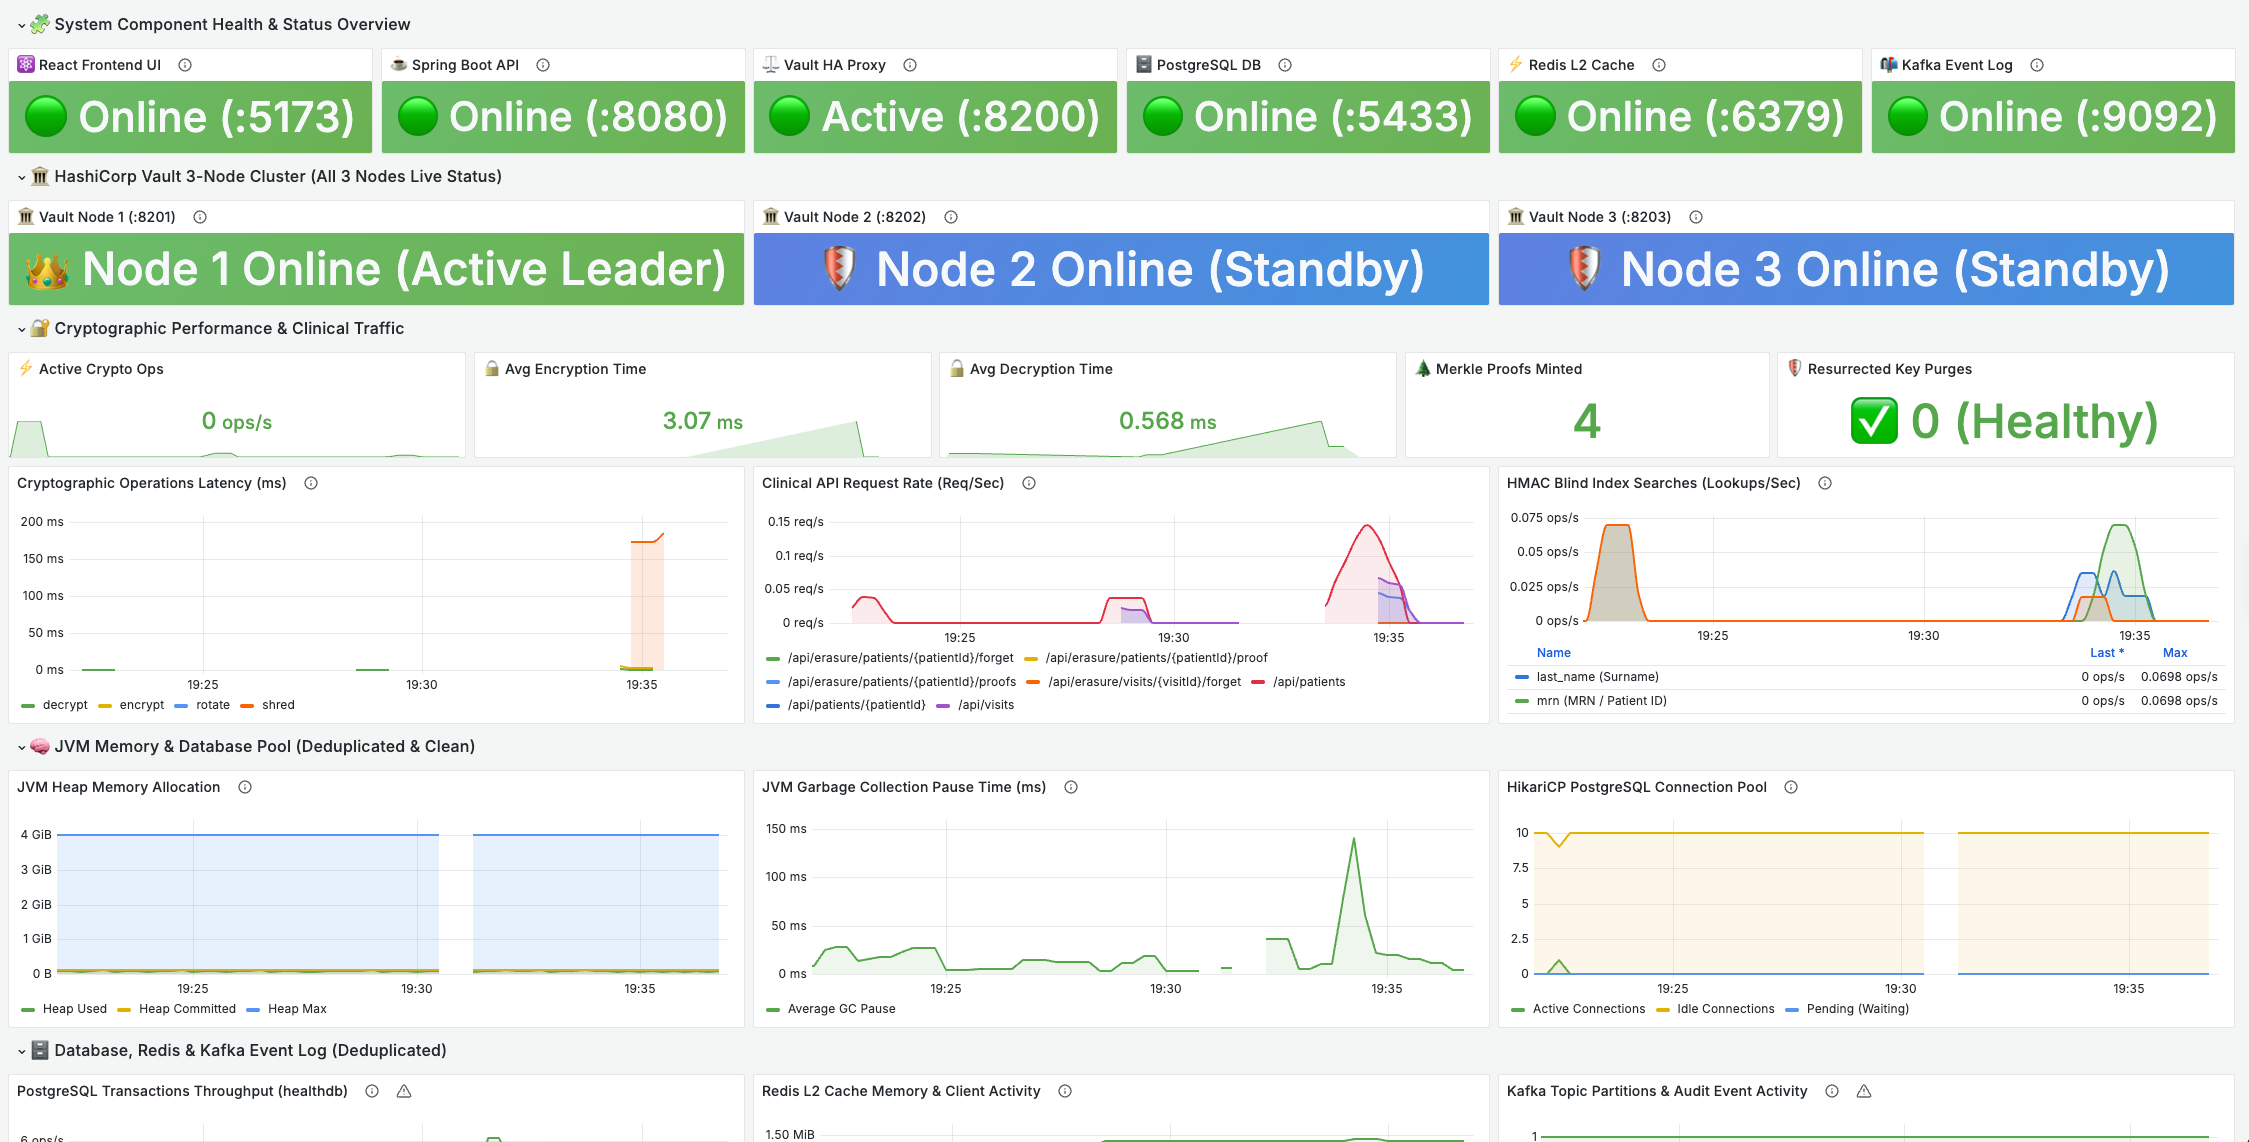
\includegraphics[width=0.95\textwidth]{images/ui_grafana_dashboard.png}
    \caption{Unified Grafana operational telemetry dashboard, correlating real-time service health across the 6-tier infrastructure with high-resolution cryptographic latency gauges and JVM memory metrics.}
    \label{fig:ui-grafana-dashboard}
\end{figure}